\subsection{Demonstration}
In this section, we will present the interface of the terrain generator, with all the features described in previous sections. 

The system has only one web page as interface. The middle of it shows the first-person view of the terrain. Below the terrain is a simple help for users to control the view. Users could move forward/backward/right/left using the arrow keys, or press 'g' to regenerate another terrain. In addition, users could toggle day or night view by pressing 'n' key. 

Figure~\ref{fig:demo_0_1} was generated using the Perlin Noise algorithm and covered by a grass texture. We could see the surface of the terrain was very smooth, with high mountains. Figure~\ref{fig:demo_1_1}, \ref{fig:demo_1_2} and \ref{fig:demo_1_3} were generated by the Diamond-square algorithm. The difference between both generated terrains was the used texture. You could also see these terrains were not as smooth as the one generated by the Perlin Noise algorithm. These generated terrains were mostly rolling hills. 

Figure~\ref{fig:demo_2_1} was generated by combining the Perlin Noise and Diamond-square algorithms. The generated terrain combines the terrain features of the two: high mountains with rough surface. Finally, the Simplex noise algorithm was used by our generator to generate sharp mountains as shown in Figure~\ref{fig:demo_3_0}, \ref{fig:demo_3_2} and \ref{fig:demo_3_3}.

\begin{figure*}
	\center
	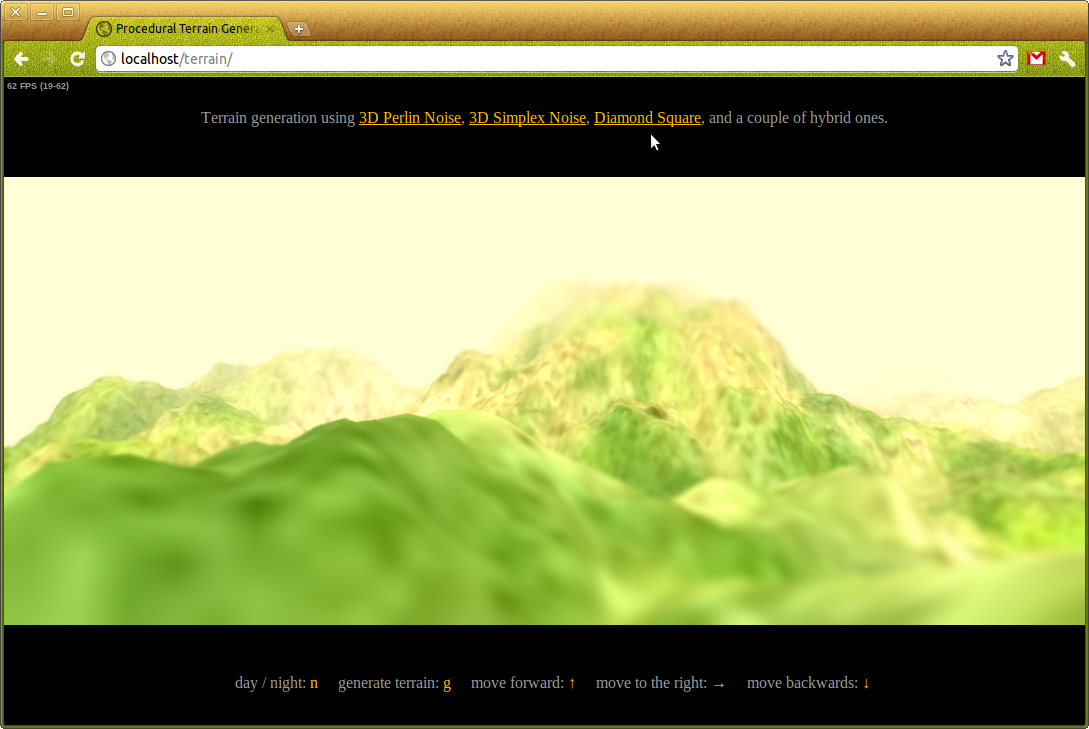
\includegraphics[scale=0.4]{images/demo_0_1.png}
	\caption{Perlin Noise with grass texture}
	\label{fig:demo_0_1}
\end{figure*}
\begin{figure*}
	\center
	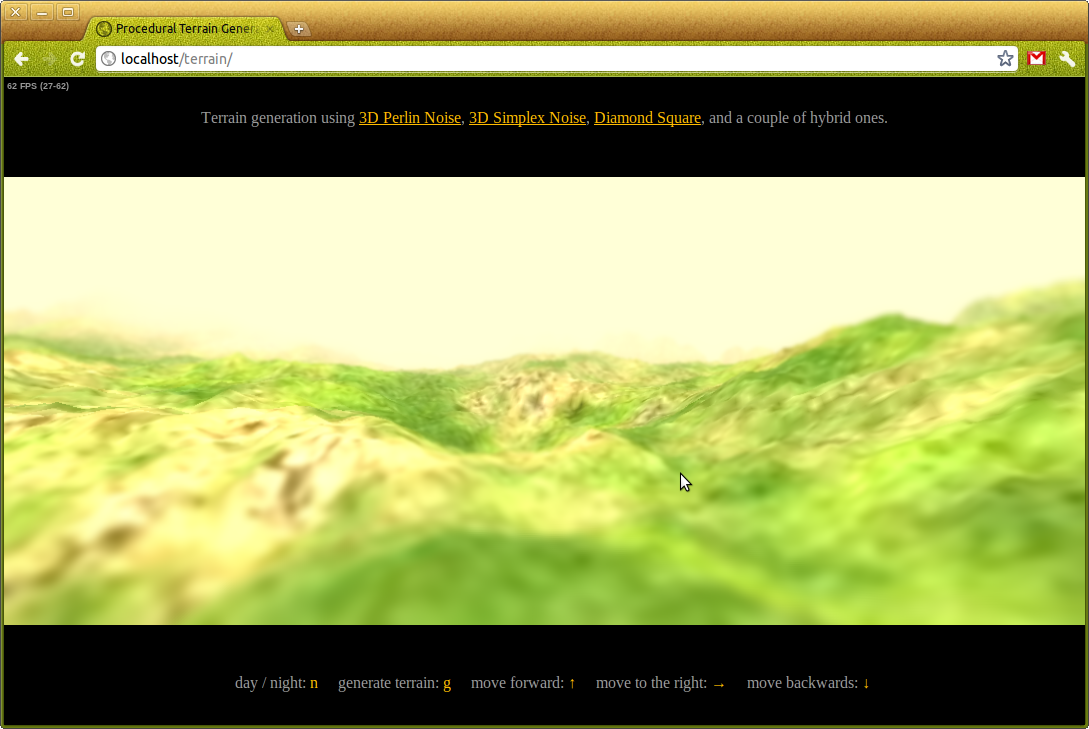
\includegraphics[scale=0.4]{images/demo_1_1.png}
	\caption{Diamond-square with grass texture}
	\label{fig:demo_1_1}
\end{figure*}
\begin{figure*}
	\center
	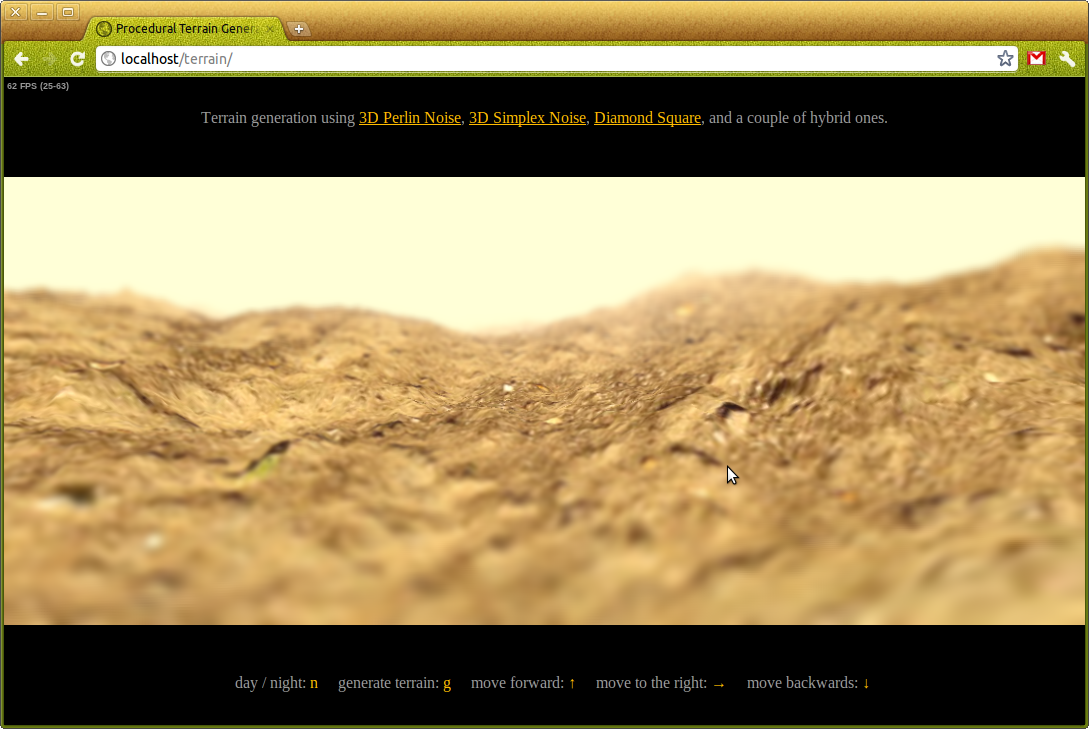
\includegraphics[scale=0.4]{images/demo_1_2.png}
	\caption{Diamond-square with sand texture}
	\label{fig:demo_1_2}
\end{figure*}
\begin{figure*}
	\center
	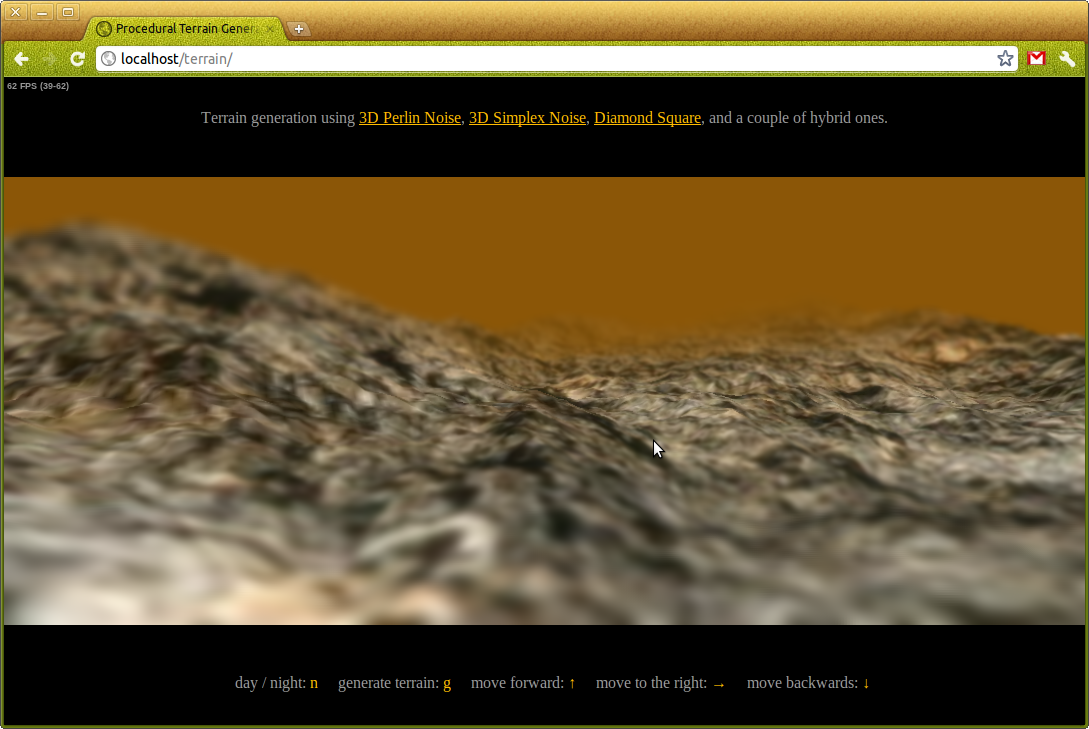
\includegraphics[scale=0.4]{images/demo_1_3.png}
	\caption{Diamond-square with rock texture}
	\label{fig:demo_1_3}
\end{figure*}
\begin{figure*}
	\center
	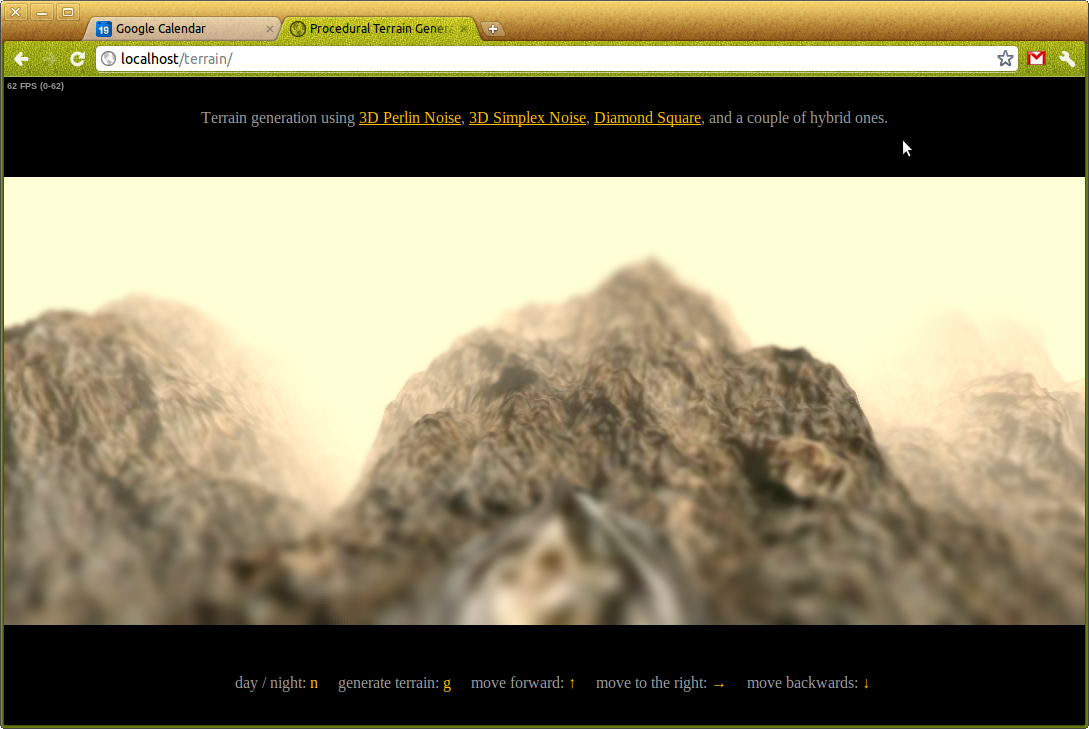
\includegraphics[scale=0.4]{images/demo_2_1.png}
	\caption{Combining Perlin noise and diamond-square with grass texture}
	\label{fig:demo_2_1}
\end{figure*}
\begin{figure*}
	\center
	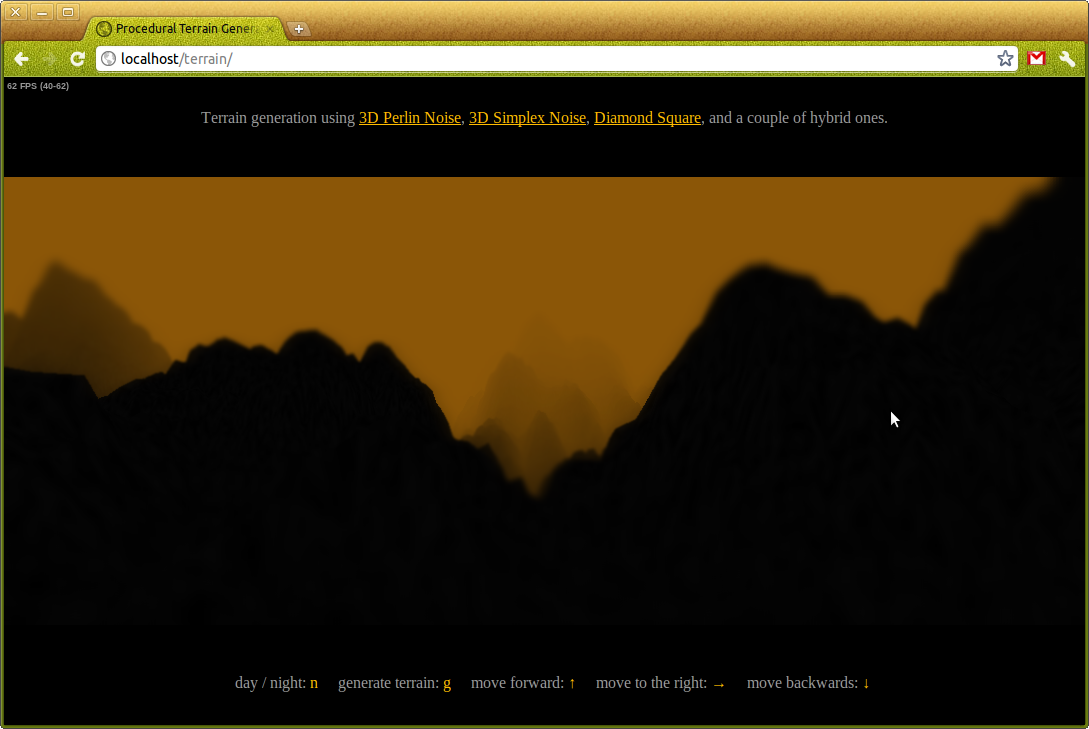
\includegraphics[scale=0.4]{images/demo_3_0.png}
	\caption{Simplex noise}
	\label{fig:demo_3_0}
\end{figure*}
\begin{figure*}
	\center
	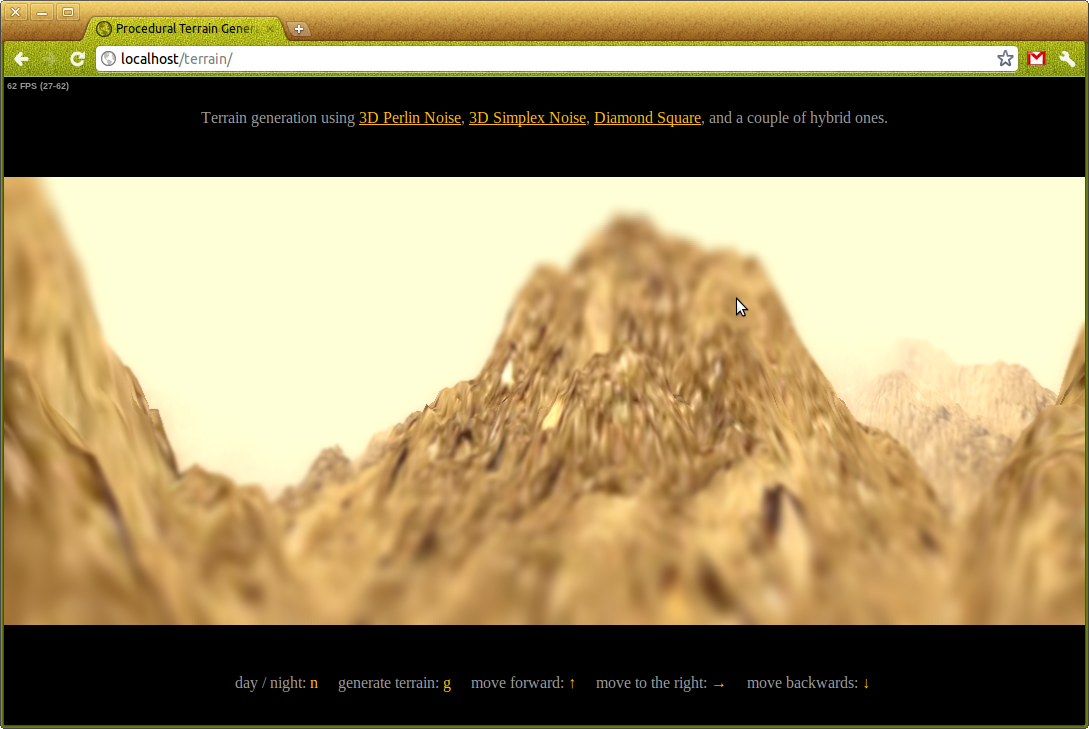
\includegraphics[scale=0.4]{images/demo_3_2.png}
	\caption{Simplex noise with sand texture}
	\label{fig:demo_3_2}
\end{figure*}
\begin{figure*}
	\center
	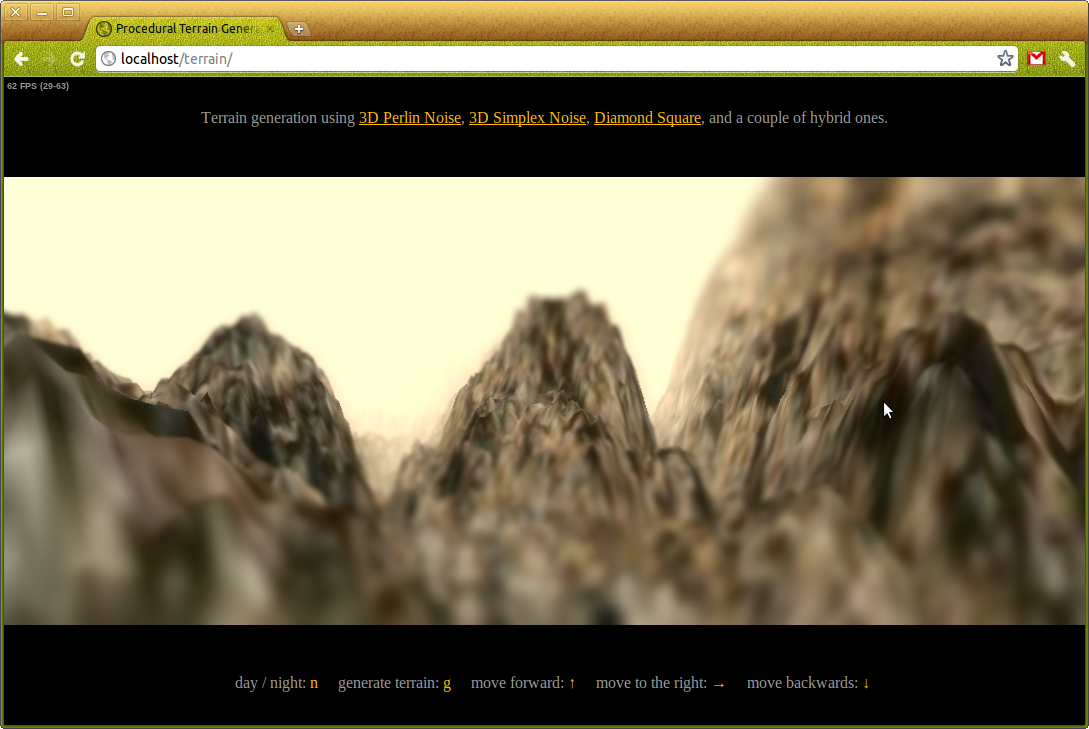
\includegraphics[scale=0.4]{images/demo_3_3.png}
	\caption{Simplex noise with rock texture}
	\label{fig:demo_3_3}
\end{figure*}
% subsection demo (end)
